\section{Объектно-ориентированный анализ}

В реультате анализа можно выделить следующие сущности:

\begin{enumerate}
\item поле
\item аргумент
\item условное выражение
\item выражение блока ON
\item выражение блока ORDER BY
\item простой запрос
\item сложный запрос
\item индекс
\end{enumerate}

Рассмотрим каждую сущность более подробно.

\subsection{Поле}
Класс \textit{Поле} представляет одну колонку таблицы.

Атрибуты:
\begin{enumerate}
\item \textit{table_number} - идентификатор таблицы
\item \textit{column_number} - идентификатор колонки
\end{enumerate}


\subsection{Аргумент}
Класс \textit{Аргумент} представляет аргумент, который используется в выражениях сравнения.

Атрибуты:
\begin{enumerate}
\item \textit{type} - тип аргумента \{value | const | null\}
\item \textit{value} - значение аргумента
\end{enumerate}


\subsection{Условное выражение}

Класс \textit{Условное выражение} представляет условное выражение, с указанием оператора сравнения и аргументов, с которыми сравнивается указанное поле.

Атрибуты:
\begin{enumerate}
\item \textit{field} - ссылка на объект класса \textit{поле},
\item \textit{operator} - оператор \{g | ge | e | ne | le | l | like\},
\item \textit{args} - массив объектов класса \textit{аргумент},
\end{enumerate}


\subsection{Выражение блока ON}
Класс \textit{Выражение блока ON} представляет выражение блока ON, где указываются два поля с оператором сравнения.

Атрибуты:
\begin{enumerate}
\item \textit{fields} - массив из двух ссылок на объекты класса \textit{поле},
\item \textit{operator} - оператор \{> | >= | = | <> | <= | < | like\},
\end{enumerate}

\subsection{Выражение блока ORDER BY}
Класс \textit{Выражение блока ORDER BY} представляет выражение блока ORDER BY, где указываются поле сортировки и направление сортировки.

Атрибуты:
\begin{enumerate}
\item \textit{field} - ссылка на объект класса \textit{поле},
\item \textit{asc} - направление сортировки, если \textit{TRUE} - то по возрастанию, иначе - по убыванию.
\end{enumerate}


\subsection{Индекс}
Класс \textit{Индекс} представляет набор полей, по которым следует построить индекс.

Атрибуты:
\begin{enumerate}
\item \textit{table_name} - имя таблицы,
\item \textit{columns_name} - имена колонок таблицы,
\item \textit{where_eq_fields} - массив ссылок на поля, по которым происходит строгое равенство,
\item \textit{where_not_eq_fields} - массив ссылок на поля, по которым происходит нестрогое равенство,
\item \textit{order_by_fields} - массив ссылок на поля, по которым происходит сортировка 
\end{enumerate}

Методы:
\begin{enumerate}
\item \textit{delete_fields([fields])} - удалить из всех атрибутов объекта \textit{индекс} поля, указанные в передаваемом массиве,
\item \textit{sql(): строка} - получить SQL строку создания индекса, при этом поля будут из \textit{where_eq_fields}, \textit{order_by_fields}, \textit{where_not_eq_fields} в порядке перечисления и с учетом правил из раздела \ref{section:simple-index} 
\end{enumerate}


\subsection{Простой запрос}
Класс \textit{Простой запрос} представляет собой распарсенный запрос в структуру программы.

Атрибуты:
\begin{enumerate}
\item \textit{sql_query} - строка с SQL запросом,
\item \textit{table_name} - имя таблицы из запроса,
\item \textit{columns_name} - имена колонок таблицы из запроса,
\item \textit{where} - массив объектов класса \textit{условное выражение},
\item \textit{order_by} - массив объектов класса \textit{выражение блока ORDER BY}.
\end{enumerate}

Методы:
\begin{enumerate}
\item \textit{init_from_sql(query)} - инициировать объект из SQL строки, т.е. по заданной SQL строке заполнить атрибуты: 
	\begin{enumerate}
	\item \textit{table_name} 
	\item \textit{columns_name}
	\item \textit{where}
	\item \textit{order_by}
	\end{enumerate}

\item \textit{get_index(): index} - создать и вернуть объект класса \textit{индекс} с помощью правил из раздела \ref{section:simple-index}
\end{enumerate}


\subsection{Сложный запрос}
Класс \textit{Сложный запрос} представляет собой распарсенный запрос в структуру программы.

Атрибуты:
\begin{enumerate}
\item \textit{sql_query} - строка с SQL запросом,
\item \textit{tables_name} - массив из двух элементов-имён таблиц из запроса,
\item \textit{columns_name} - массив из двух элементов-массивов имён колонок таблиц из запроса,
\item \textit{join_type} - тип соединения таблиц \{inner | left | right\}
\item \textit{on} - массив объектов класса \textit{выражение блока ON},
\item \textit{where} - массив объектов класса \textit{условное выражение},
\item \textit{order_by} - массив объектов класса \textit{выражение блока ORDER BY}.
\end{enumerate}

Методы:
\begin{enumerate}
\item \textit{init_from_sql(query)} - инициировать объект из SQL строки,
\item \textit{get_optimization_join(): join_type} - получить тип join, который будет использован оптимизатором MySQL (см. раздел \ref{section:fullscan}),
\item \textit{get_fullscan_table(): table_number} - определить по какой таблице будет осуществлено полное сканирование,
\item \textit{get_simple_queries(): simple_query_1, simple_query_2} - разбить запрос на два простых подзапоса,
\item \textit{get_indexes(): [indexes]} - вернуть индексы этого запроса.
\end{enumerate}

\subsection{Диаграмма классов}

Выделенные сущности можно представить на диаграмме классов на рисунке \ref{img:diag-class}

\begin{figure}[h!]
  \centering
  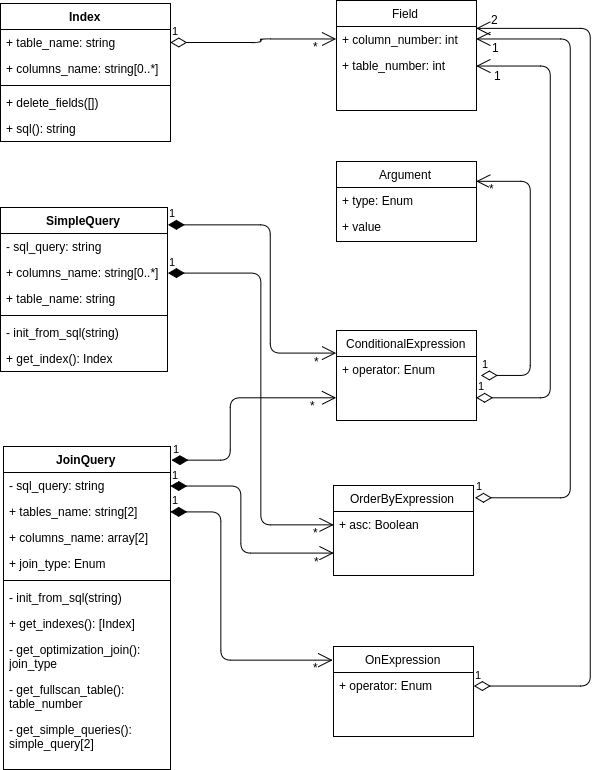
\includegraphics[scale=0.7]{diag-class.png}
  \caption{Диаграмма классов}
  \label{img:diag-class}
\end{figure}
